\chapter{MODELADO DEL SISTEMA NO LINEAL Y LINEAL DE LA PLATAFORMA STEWART}
\label{cap:modeladoStewart}
\markboth{CAPÍTULO \thechapter. MODELADO PLATAFORMA STEWART}{CAPÍTULO \thechapter. MODELADO PLATAFORMA STEWART}

El presente capítulo tiene como principal objetivo describir el modelo no lineal de la plataforma Stewart, con sus dinámicas internas y bloques necesarios para el futuro control de la misma. Además, se desarrolla la linealización de la plataforma, factor primordial para el diseño de control en los capítulos siguientes.


%##############################################################
%##############################################################
\section{Modelo no lineal de la plataforma Stewart}
\lhead[\thepage]{Sección \thesection. Modelo No Lineal}

El modelado de una plataforma Stewart se comprende principalmente por un conjunto de bloques encargados de facilitar el manejo y control de la plataforma. Se puede observar en la Figura \ref{fig:stewart_scheme} los bloques principales del modelado de la plataforma Stewart.

\begin{figure}[ht]
\centering
    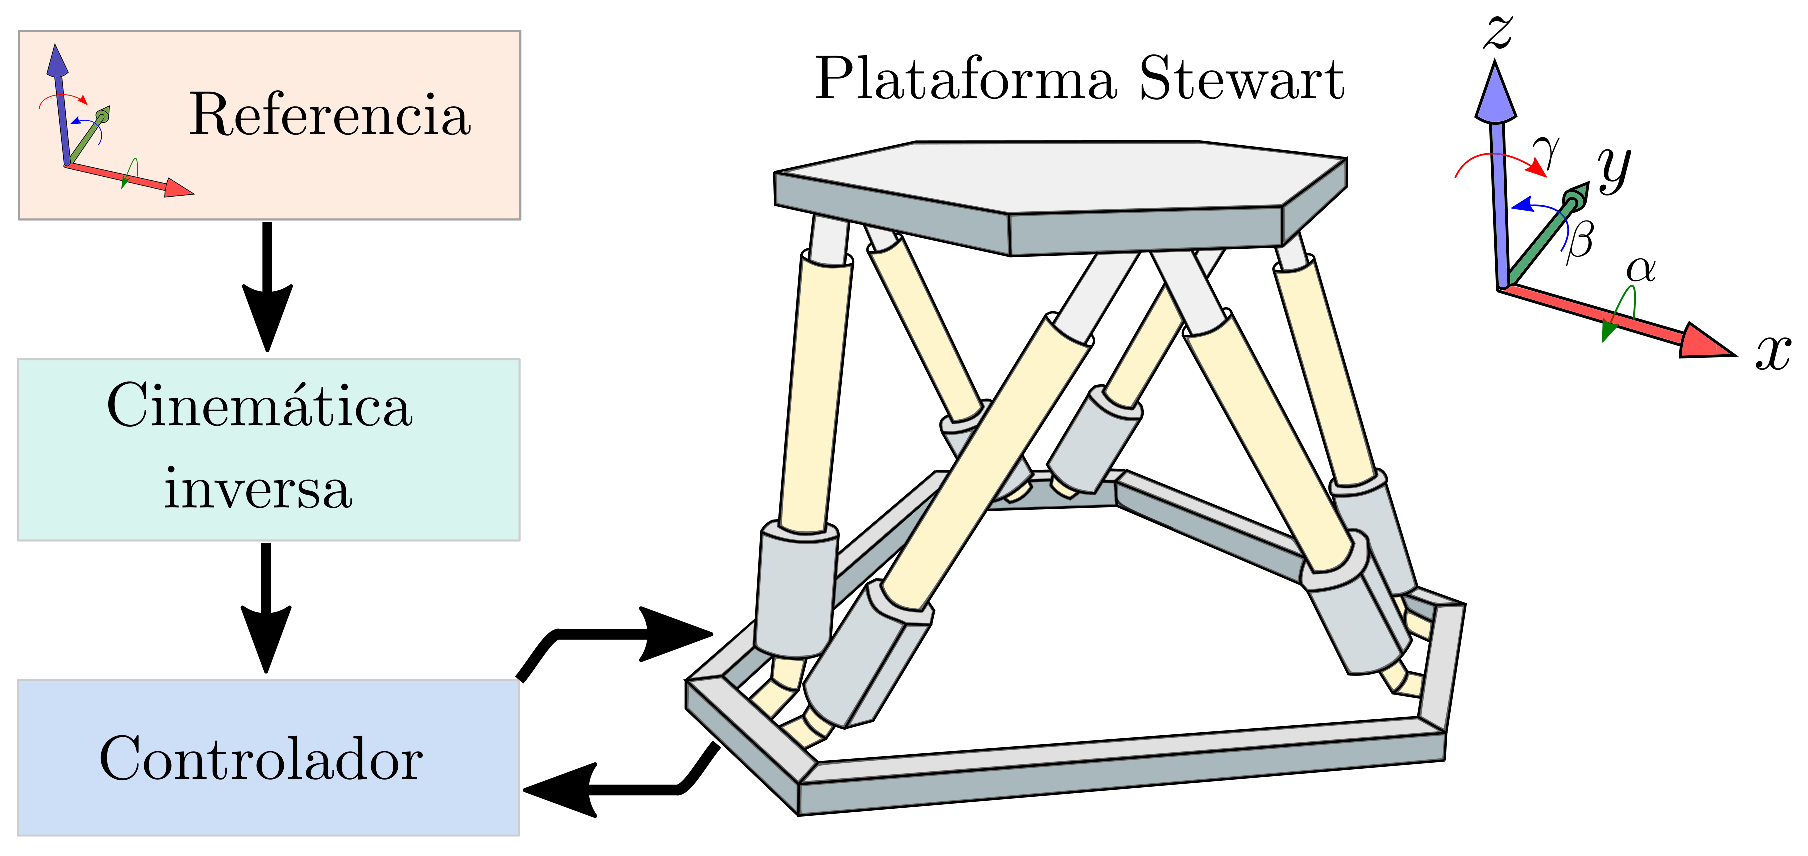
\includegraphics[width=0.6\columnwidth]{Figures/stewart_scheme.eps}
    \caption{Esquema de una plataforma Stewart.}
    \label{fig:stewart_scheme}
\end{figure}



\subsection{Bloque Referencia}

El primer bloque corresponde a la referencia global que se desea de la plataforma Stewart, es decir, describir el movimiento del centro de masa de la plataforma superior. Este movimiento describe el desplazamiento del centro de masa en los ejes $x$, $y$, $z$ representados por $P_x$, $P_y$, $P_z$, así como los movimientos de rotación de estos mismos ejes denotados como $\alpha, \beta, \gamma$.

\begin{equation} \label{eq:ref}
    q_{ref} = \begin{bmatrix}
        P_x & P_y & P_z & \alpha & \beta & \gamma
    \end{bmatrix}^{\top}
\end{equation}


\subsection{Bloque Cinemática Inversa}

El bloque de Cinemática Inversa es uno de los más importantes, ya que es el encargado de transformar el movimiento deseado del centro de masa de la plataforma superior ($q_{ref}$), al desplazamiento lineal deseado por cada brazo actuador. El análisis completo de este bloque se basa en el trabajo de \textit{Zafer Bingul y Oguzhan Karahan} en \cite{bingul2012modeling}.

\subsubsection{Largo de Brazos}

Se ilustran los puntos de conexión de los brazos entre ambas plataformas (base $B$ y superior $T$) en la Figura \ref{fig:stewart_ejes}, además de sus respectivos ejes de coordenada. Los puntos $B_i$ corresponden a las conexiones en la base, mientras que los puntos $T_i$ corresponden a los de la plataforma superior, con $i = 1,...,6 \in \mathbb{N} $.

\begin{figure}[ht]
\centering
    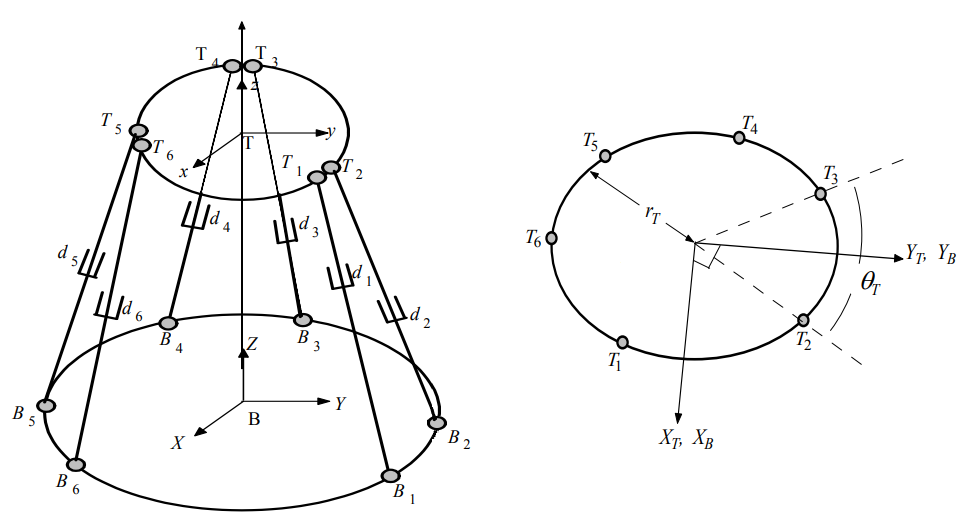
\includegraphics[width=0.8\columnwidth]{Figures/stewart_ejes.png}
    \caption{Diagrama esquemático de la plataforma Stewart (Imagen obtenida de [20]).}
    \label{fig:stewart_ejes}
\end{figure}

También desde la Figura \ref{fig:stewart_ejes} se definen los ángulos de separación entre los puntos de fijación de cada plataforma, es decir, $\theta_{T}$ para los ángulos de la plataforma superior y $\theta_{B}$ para la base. Además se define el radio de cada plataforma como $r_{T}$ y $r_{B}$ para la plataforma superior y de la base respectivamente.

Con los parámetros definidos anteriormente, se procede a modelar cada punto de conexión de la plataforma superior y de la base a sus respectivos ejes de coordenadas, mediante sus coordenadas polares de la forma:

\begin{equation}
    T_i = \begin{bmatrix} 
            T_{xi} \\ T_{yi} \\ T_{zi} 
        \end{bmatrix} = 
        \begin{bmatrix}
            r_{T} \cdot cos(\lambda_i) \\ r_{T} \cdot sin(\lambda_i) \\ 0 
        \end{bmatrix} , \quad \textrm{con} \quad
        \begin{array}{lcc}
            \lambda_i = \frac{i\pi}{3} - \frac{\theta_{T}}{2} & \textrm{para} & i=1,3,5\\
            \lambda_i = \lambda_{i-1}+\theta_{T} & \textrm{para} & i=2,4,6
        \end{array}
\end{equation}

\begin{equation}
    B_i = \begin{bmatrix} 
        B_{xi} \\ B_{yi} \\ B_{zi} 
    \end{bmatrix} = 
    \begin{bmatrix} 
        r_{B} \cdot cos(\upsilon_i) \\ r_{B} \cdot sin(\upsilon_i) \\ 0 
    \end{bmatrix} , \quad \textrm{con} \quad
    \begin{array}{lcc}
         \upsilon_i = \frac{i\pi}{3} - \frac{\theta_{B}}{2} & \textrm{para} & i=1,3,5 \\
         \upsilon_i = \upsilon_{i-1}+\theta_{B} & \textrm{para} & i=2,4,6
    \end{array}
\end{equation}

Una vez definido los puntos de conexión de ambas plataformas, se debe describir una matriz de rotación $R_{T}^{B}$ definida por los ángulos de rotación del centro de masa superior ($\alpha, \beta, \gamma$), encargada de convertir la rotación de la plataforma superior a el eje de la base. 

\begin{equation}
    R_T^B(\alpha,\beta,\gamma) = \begin{bmatrix}
        c_\beta c_\gamma & c_\gamma s_\alpha s_\beta - c_\alpha s_\gamma & s_\alpha s_\gamma + c_\alpha c_\gamma s_\beta \\
        c_\beta c_\gamma & c_\alpha c_\gamma + s_\alpha s_\beta s_\gamma & c_\alpha s_\beta s_\gamma - c_\gamma s_\alpha \\
        -s_\beta & c_\beta s_\alpha & c_\alpha c_\beta \\
    \end{bmatrix}
\end{equation}

donde $c_\alpha$, $c_\beta$ y $c_\gamma$ son abreviaciones para $cos(\alpha)$, $cos(\beta)$ y $cos(\gamma)$ respectivamente. Similarmente $s_\alpha$, $s_\beta$ y $s_\gamma$ denotan el seno de los ángulos de rotación $\alpha$, $\beta$ y $\gamma$.\\

Por otro lado, el vector $P$ de traslación del origen de la plataforma superior con respecto a la base, se define con los primeros términos de la referencia $q_{ref}$ (\ref{eq:ref}) que describen el desplazamiento lineal del eje superior.

\begin{equation}
    P = \begin{bmatrix}
        P_x & P_y & P_z
    \end{bmatrix}^{\top}
\end{equation}

De esta forma, mediante los puntos de conexión de la plataforma superior $T_i$ y de la base $B_i$, con la matriz de rotación $R_T^B$ y el vector $P$ de traslación del origen de la plataforma superior, se define el vector $L_i$ que describe el movimiento de cada brazo actuador en forma vectorial:

\begin{equation}
    L_i = R_T^B T_i + P - B_i
\end{equation}

El largo respectivo de cada brazo se define entonces como:

\begin{equation}
    l_i = \norm{L_i}_2 \quad \textrm{para} \quad i=1,...,6
\end{equation}



\subsubsection{Velocidad de Brazos (Matriz Jacobiana)}

La matriz Jacobiana es la encargada de relacionar las velocidades de cada brazo actuador a la velocidad de movimiento de la plataforma superior. Para los manipuladores paralelos se suele usar la matriz Jacobiana como:

\begin{equation}
    \dot{L} = \mathcal{J} \dot{X}
\end{equation}
donde $\dot{L}$ y $\dot{X}$ corresponden a la velocidad de los brazos y de la plataforma superior respectivamente, y $\mathcal{J}$ representa a la matriz Jacobiana.

Esta matriz Jacobiana se puede separar en 2 matrices distintas, de la forma:

\begin{equation}
    \mathcal{J} = \mathcal{J}_1 \mathcal{J}_2
\end{equation}

Para la obtención de estas matrices mencionadas, se debe analizar la vista esquemática de los brazos de la plataforma Stewart, mostrada en la Figura \ref{fig:leg_scheme}. 

\begin{figure}[ht]
\centering
    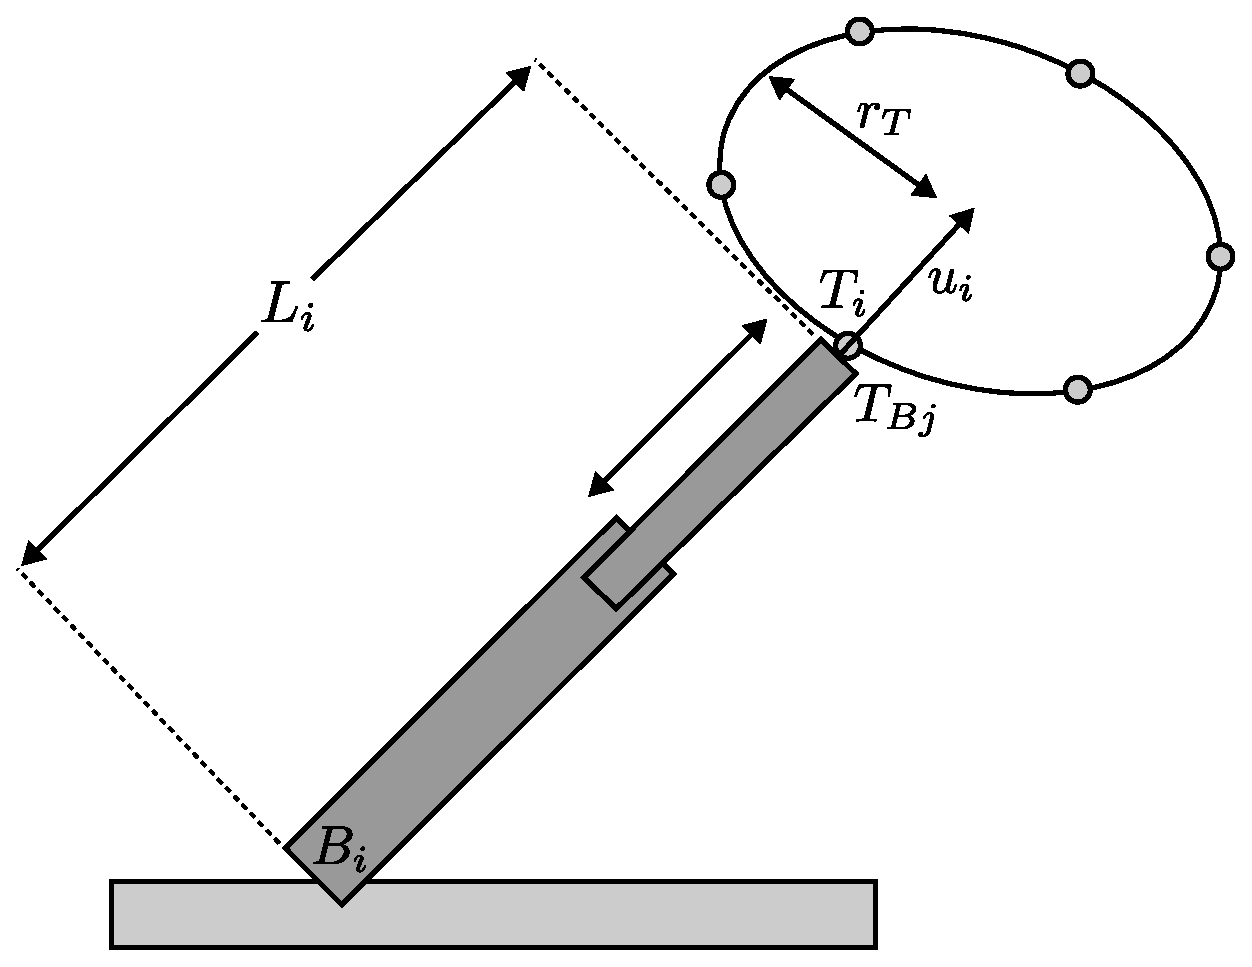
\includegraphics[width=0.5\columnwidth]{Figures/leg_scheme.eps}
    \caption{Vista esquemática de los brazos de la plataforma Stewart (Imagen obtenida de [20]).}
    \label{fig:leg_scheme}
\end{figure}

Dados los puntos de conexión $T_i$ de la plataforma superior respecto a su propio eje, de la Figura \ref{fig:leg_scheme} es posible definir $T_{Bj}$ como los puntos de conexión de la plataforma superior con referencia al sistema de coordenadas de la base dado por:
\begin{equation} \label{UpJoint_base}
    T_{Bj} = \begin{bmatrix}
        P_x & P_y & P_z
    \end{bmatrix}^{\top} + R_T^B T_i = P + R_T^B T_i
\end{equation}
donde $P$ el vector de traslación del origen de la plataforma superior respecto a la base y $R_T^B$ la matriz de rotación, definidos anteriormente.

Además, se define $\vec{u}_i$ como el vector unitario a lo largo del eje de la junta prismática de la conexión superior, de la forma:
\begin{equation}
    \vec{u}_i = \frac{B_i T_{Bj}}{\abs{L_i}} = \frac{L_i}{l_i} , \begin{cases}
        j = \frac{i+1}{2} & \textrm{si } i \textrm{ es impar}\\
        j = \frac{i}{2} & \textrm{si } i \textrm{ es par}
    \end{cases}
\end{equation}

Una vez definido los parámetros anteriores, es posible obtener la velocidad de los puntos de conexión $T_{Bj}$ derivando la ecuación \ref{UpJoint_base} con respecto al tiempo, obteniendo: 
\begin{equation}
    \vec{V}_{T_{Bj}} = \dot{T}_{Bj} = \begin{bmatrix}
        \dot{P}_x & \dot{P}_y & \dot{P}_z
    \end{bmatrix}^{\top} 
    + w \times R_T^B T_i = \dot{P} + w \times R_T^B T_i
\end{equation}
donde $w=(w_x, w_y, w_Z)$ es la velocidad angular de la plataforma superior con referencia a la base. 

\begin{equation}
    w = \begin{bmatrix}
        w_x \\ w_y \\ w_z
    \end{bmatrix}
    = \begin{bmatrix}
        cos(\beta) & 0 & 0 \\
        0 & 1 & -sin(\alpha)\\
        -sin(\beta) & 0 & cos(\alpha)
    \end{bmatrix}
    = \begin{bmatrix}
        \dot{\alpha} \\ \dot{\beta} \\ \dot{\gamma}
    \end{bmatrix}
\end{equation} 

Dado que, la proyección del vector velocidad $\vec{V}_{T_{Bj}}$ (ó $\dot{T}_{Bj}$) sobre el eje de la proyección prismática $\vec{u}_i$ de las conexiones produce la tasa de extensión de la conexión $i$, entonces es posible definir la velocidad activa $\dot{L}_i$ de los brazos actuadores como:
\begin{equation} \label{eq:leg_velocity1}
    \dot{L}_i = \vec{V}_{Bj} \vec{u}_i =  \begin{bmatrix}
        \dot{P}_x & \dot{P}_y & \dot{P}_z
    \end{bmatrix}^{\top} \cdot \vec{u}_i
    + w \times \left(R_T^B T_i \right) \cdot \vec{u}_i = \dot{P} \cdot \vec{u}_i + w \times \left(R_T^B T_i\right) \cdot \vec{u}_i
\end{equation}

Reescribiendo la ecuación \ref{eq:leg_velocity1} de forma matricial se obtiene:
\begin{equation}
    \dot{L}_i = \mathcal{J} \begin{bmatrix}
        \dot{P} \\ w
    \end{bmatrix} =
    \mathcal{J} \cdot \dot{q}_{ref} = \mathcal{J}_1 \mathcal{J}_2 \cdot \dot{q}_{ref}
\end{equation}

donde $\dot{q}_{ref}$ es la derivada del desplazamiento y orientación deseada de la plataforma superior, con las matrices Jacobianas $\mathcal{J}_1$ y $\mathcal{J}_2$ descritas como:
\begin{equation}
    \mathcal{J}_1 = \begin{bmatrix}
        u_{x1} & u_{y1} & u_{z1} & \left( R_T^B T_1 P \vec{u}_1 \right)^{\top} \\
        \vdots & \vdots & \vdots & \vdots \\
        u_{x6} & u_{y6} & u_{z6} & \left( R_T^B T_6 P \vec{u}_6 \right)^{\top} 
    \end{bmatrix}_{6\times6}
\end{equation}

\begin{equation}
    \mathcal{J}_2 = \begin{bmatrix}
        1 & 0 & 0 & 0 & 0 & 0 \\
        0 & 1 & 0 & 0 & 0 & 0 \\
        0 & 0 & 1 & 0 & 0 & 0 \\
        0 & 0 & 0 & cos(\beta) & 0 & 0\\
        0 & 0 & 0 & 0 & 1 & -sin(\alpha)\\
        0 & 0 & 0 & -sin(\beta) & 0 & cos(\alpha)
    \end{bmatrix}
\end{equation}


\subsection{Modelo Dinámico}

El análisis de las ecuaciones del modelo dinámico de la plataforma Stewart no es algo sencillo debido a la existencia de muchas cinemáticas relacionadas con la estructura de los brazos y de las plataformas, que a la vez, al estar todo conectado entre si, el efecto que se produce entre ellas es significativo. Se han descrito diversos tipos de métodos para describir la dinámica de la plataforma Stewart, pero no hay un consenso sobre cual es el más efectivo. 

En \cite{bingul2012modeling} se desarrolla el análisis a través de las energías cinéticas y potenciales de la plataforma superior y de los 6 brazos actuadores, que en conjunto, logran describir de forma general la energía cinética y potencial de la plataforma Stewart.\\

El comportamiento del sistema se basa en las ecuaciones de Euler-Lagrange aplicadas a la plataforma Stewart. A través del movimiento generalizado ($q$) de la plataforma superior y de las fuerzas generalizadas ($\tau$) aplicadas, junto a la energía cinética $E_K(q,\dot{q})$ y potencial $E_P(q)$ general de la plataforma Stewart, se define la ecuación dinámica del sistema como:
\begin{equation} \label{eq:dinamic1}
    \frac{d}{dt} \frac{dL}{d \dot{q}} - \frac{\partial L}{\partial q} = \frac{d}{dt} \left( \frac{\partial E_K(q,\dot{q})}{\partial \dot{q}} \right) - \frac{\partial E_K(q,\dot{q})}{\partial q} + \frac{\partial E_P(q)}{\partial q} = \tau
\end{equation}

Reemplazando las variables generales anteriores $q$ y $\tau$ por el movimiento deseado de la plataforma superior $q_{ref}$ y las fuerzas reales aplicadas por los actuadores, se deriva de \ref{eq:dinamic1} la ecuación dinámica como:

\begin{equation} \label{eq:dinamic2}
    M(q_{ref}) \Ddot{q}_{ref} + H(q_{ref},\dot{q}_{ref}) \dot{q}_{ref} + G(q_{ref}) = \mathcal{J}(q_{ref})^{\top} F
\end{equation}

donde $M(q_{ref})$ es la matriz de inercia, $H(q_{ref},\dot{q}_{ref})$ es la matriz Coriolis-Centrifugal y $G(q_{ref})$ es la matriz de gravedad de la plataforma móvil y brazos. Además, $\mathcal{J}(q_{ref})$ es la matriz Jacobiana y $F=\begin{bmatrix} f_1 & f_2 & f_3 & f_4 & f_5 & f_6 \end{bmatrix}^T$ con $f_i$ la fuerza aplicada por el actuador del brazo $i$ en la dirección de proyección $\vec{u}_i$ de las conexiones entre los brazos y la plataforma superior.


\subsection{Simulación Modelo No Lineal}

Se utiliza un modelo mecánico desarrollado por \textit{MathWorks} en \textit{Simscape Multibody} para el programa \textit{Matlab/Simulink}, el cual se conforma de una serie de bloques conectados entre si, representando los elementos físicos de la plataforma.

Este tipo de modelo mecánico es utilizado ampliamente ya que posee integradas las ecuaciones dinámicas del sistema, además de no linealidades, interacciones y otro tipo de fenómenos entre componentes que en los modelos matemáticos simples no están presentes. De esta forma se garantiza así un modelo más confiable y realista. Otro beneficio de este modelo mecánico es que proporciona una vista recreativa de la maquina en 3D, mostrando los movimientos y comportamientos visuales de la plataforma Stewart de forma cinematográfica. 

En la Figura \ref{fig:sim_slk_general} es posible apreciar el modelo mecánico utilizado en \textit{Matlab/Simulink}, además de sus bloques internos que lo componen y la ventana cinematográfica 3D para observar los movimientos de la plataforma.

%%%%%%%%%%%%%%% FIGURA MODELO NO LINEAL %%%%%%%%%%%%%%%%%%%%%

%##############################################################
%##############################################################

\section{Linealización de modelo no lineal de la plataforma Stewart}
\lhead[\thepage]{Sección \thesection. Linealización de modelo}
\label{sec:linealizacion_stewart}

Debido a la no linealidad del sistema, su comportamiento con respecto a una variable dada es muy impredecible, por ende, para poder diseñar un control confiable se necesita de una aproximación lineal del sistema. Para esto, se estudia la estabilidad del sistema en torno a un punto de operación. 

\subsection{Punto de Operación}

Para la obtención del punto de operación del sistema se utilizan los mismos bloques mencionados anteriormente, más específicamente los mostrados en las Figuras \ref{fig:sim_slk_general1} y \ref{fig:sim_slk_general3}. 

Se edita el bloque que describe el comportamiento de los brazos actuadores, de tal forma que la entrada sea el largo de cada brazo y que la salida sea el torque necesitado por cada actuador para mantener tal posición. En la Figura \ref{fig:sim_slk_eq} se aprecia el bloque general modificado del modelo mecánico (Figura \ref{fig:sim_slk_eq_general}) y el bloque interno modificado de cada brazo actuador con su configuración correspondiente (Figura \ref{fig:sim_slk_eq_legconfig}).

%%%%%%%%%%%%%%% FIGURA PUNTO DE OPERACION %%%%%%%%%%%%%%%%%%%%%

Se toma como punto de operación, la posición de \textit{reposo} de la plataforma en la cual los brazos no poseen extensión alguna, es decir para un largo de $0(cm)$, y la fuerza necesaria para mantener tal posición. De esta forma se describe el punto de operación definido como $(l_{EQ},\tau_{EQ})$: 

\begin{equation}
    l_{EQ} = \begin{bmatrix} 0 \\ \vdots \\ 0 \end{bmatrix}_{6\times1} \hspace{0.5cm} \Longrightarrow \hspace{0.5cm} \tau_{EQ} = \begin{bmatrix} 36.987 \\ \vdots \\ 36.987\end{bmatrix}_{6\times1}
\end{equation}

%%%%%%%%%%%%%%% FIGURA MODELO NO LINEAL %%%%%%%%%%%%%%%%%%%%%
\begin{figure}[H]
    \centering
    \begin{subfigure}[b]{0.4\textwidth}
        \centering
        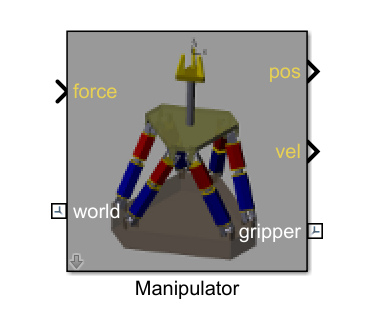
\includegraphics[width=1\columnwidth]{Figures/stewart_simulink1.png}
        \caption{Bloque general del modelo mecánico.}
        \label{fig:sim_slk_general1}
    \end{subfigure}
    \hfill
    \begin{subfigure}[b]{0.4\textwidth}
       \centering
        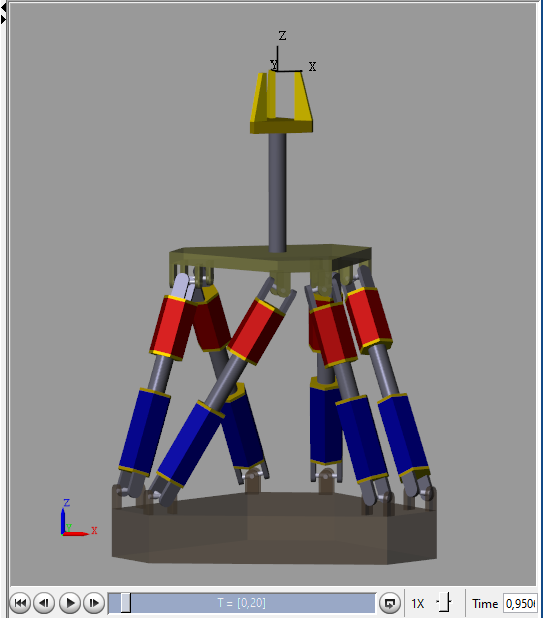
\includegraphics[width=0.75\columnwidth]{Figures/stewart_simulink3.png}
        \caption{Ventana cinematográfica 3D.}
        \label{fig:sim_slk_general2}
    \end{subfigure}
    \hfill
    \begin{subfigure}[b]{\textwidth}
       \centering
        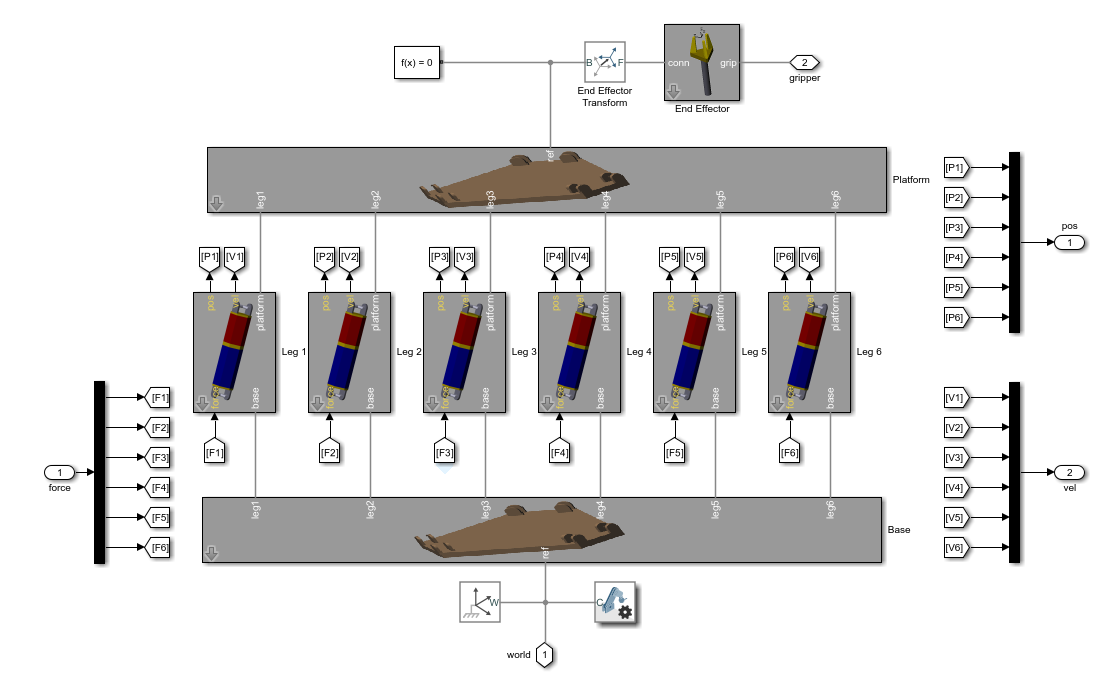
\includegraphics[width=1\columnwidth]{Figures/stewart_simulink2.png}
        \caption{Bloques internos del modelo mecánico.}
        \label{fig:sim_slk_general3}
    \end{subfigure}
    \caption{Bloques de simulación Matlab/Simulink para plataforma Stewart.}
    \label{fig:sim_slk_general}
\end{figure}

%%%%%%%%%%%%%%% FIGURA PUNTO DE OPERACION %%%%%%%%%%%%%%%%%%%%%
\begin{figure}[H]
    \centering
    \begin{subfigure}[b]{\textwidth}
        \centering
        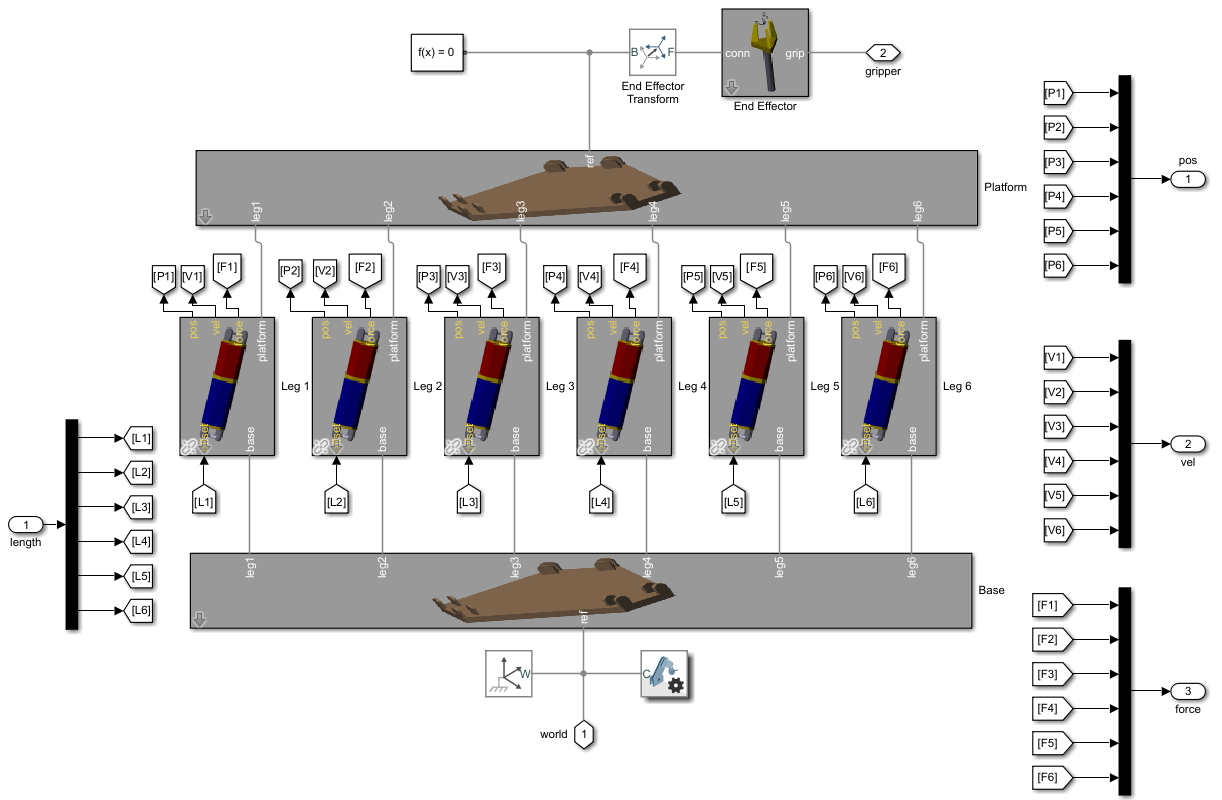
\includegraphics[width=0.85\columnwidth]{Figures/sim_slk_eq_general.png}
        \caption{Bloque general modificado del modelo mecánico para obtención del punto de operación.}
        \label{fig:sim_slk_eq_general}
    \end{subfigure}
    \hfill
    \begin{subfigure}[b]{\textwidth}
       \centering
        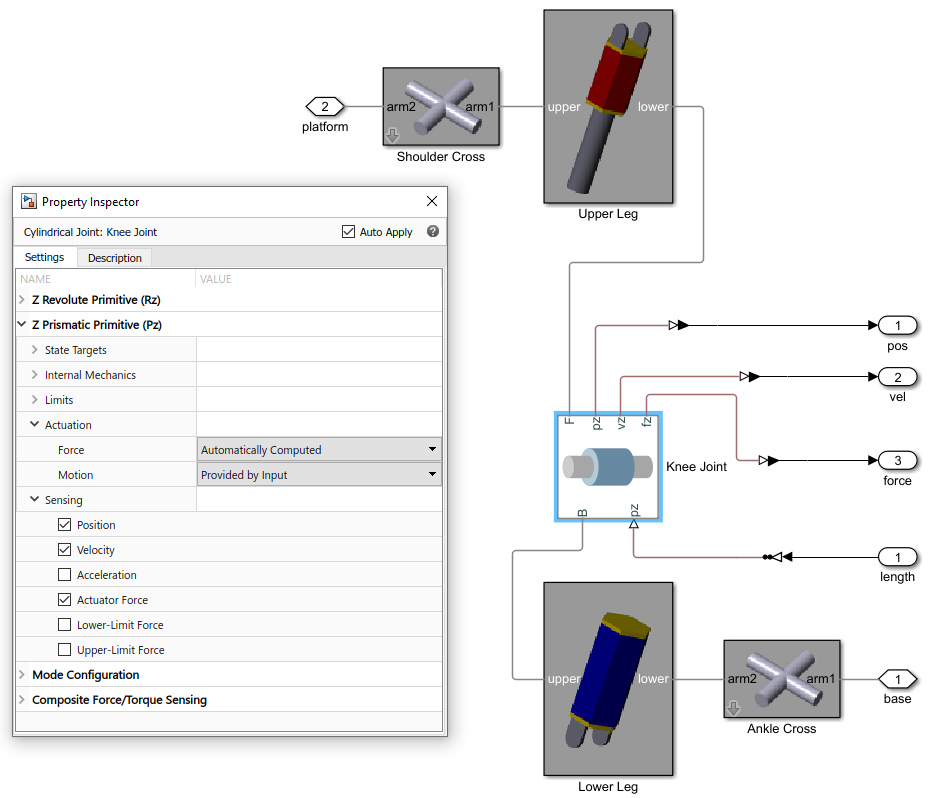
\includegraphics[width=0.7\columnwidth]{Figures/sim_slk_eq_legconfig.png}
        \caption{Configuración brazos actuadores para obtención del punto de operación.}
        \label{fig:sim_slk_eq_legconfig}
    \end{subfigure}
    \caption{Bloques de simulación Matlab/Simulink modificados para obtención del punto de operación.}
    \label{fig:sim_slk_eq}
\end{figure}


\subsection{Linealización}

Una vez obtenido el punto de operación, se procede a la linealización del sistema no lineal. Para esto, se utiliza una función llamada \textit{linmod()} que recibe como argumentos la Figura del bloque Simulink del modelo mecánico original \ref{fig:sim_slk_general1} y el punto de operación $(l_{EQ},\tau_{EQ})$ obtenido anteriormente.

De esta forma, se obtiene el modelo linealizado de la plataforma Stewart en formato de variables de estados: 
\begin{subequations} \label{eq:sys_varestados_original}
    \begin{align}
        \Dot{x}(t) & = A x(t) + B u(t), \\
        y(t) & = C x(t) + D u(t)
    \end{align}    
\end{subequations}

donde el vector de estados esta ordenado como $x(t) = \begin{bmatrix} x_1(t) & \dot{x}_1(t) & \hdots & x_6(t) & \dot{x}_6(t) \end{bmatrix}^{\top}$, el vector de entrada es de la forma $u(t) = \begin{bmatrix} u_1(t) & \hdots & u_6(t) \end{bmatrix}^{\top}$ y las matrices $A,B,C,D$ son

\begin{equation}
    A = \scalebox{0.95}{$\begin{bmatrix}
        0 &	1 &	0 &	0 &	0 &	0 &	0 &	0 &	0 &	0 &	0 &	0 \\
        32.623 & 0 & 18.85 & 0 & \textrm{-}12.29 & 0 & 8.51 & 0 & 32.49 & 0 & 25.75 & 0 \\
        0 &	0 &	0 &	1 &	0 &	0 &	0 &	0 &	0 &	0 &	0 &	0 \\
        19.83 &	0 &	28.61 &	0 &	1.27 &	0 &	17.93 &	0 &	28.20 &	0 &	30.97 &	0 \\
        0 &	0 &	0 &	0 &	0 &	1 &	0 &	0 &	0 &	0 &	0 &	0 \\
        \textrm{-}10.66 & 0 & 17.56 & 0 & 56.32 & 0 & \textrm{-}12.49 & 0 & \textrm{-}29.41 & 0 & 20.13 & 0 \\
        0 &	0 &	0 &	0 &	0 &	0 &	0 &	1 &	0 &	0 &	0 &	0 \\
        \textrm{-}5.19 &	0 &	\textrm{-}6.83 &	0 &	\textrm{-}7.23 &	0 &	75.76 &	0 &	9.66 &	0 &	24.39 &	0 \\
        0 &	0 &	0 &	0 &	0 &	0 &	0 &	0 &	0 &	1 &	0 &	0 \\
        3.08 & 0 & 9.72 & 0 & \textrm{-}2.61 & 0 & \textrm{-}13.57 & 0 & 34.10 & 0 & 0.69 & 0 \\
        0 &	0 &	0 &	0 &	0 &	0 &	0 &	0 &	0 &	0 &	0 &	1 \\
        6.56 & 0 & 3.36 & 0 & 10.21 & 0 & \textrm{-}4.67 & 0 & \textrm{-}0.23 & 0 & 35.91 & 0 \\
    \end{bmatrix}$}
\end{equation}

\begin{equation}
    B = \scalebox{0.95}{$\begin{bmatrix}
        0 &	0 &	0 &	0 &	0 &	0 \\
        0.070 &	0.333 &	\textrm{-}0.658 & \textrm{-}0.465 & 0.436 & 0.673 \\
        0 &	0 &	0 &	0 &	0 &	0 \\
        \textrm{-}0.333 &	\textrm{-}0.070 &	\textrm{-}0.673 &	\textrm{-}0.436 &	0.465 &	0.658 \\
        0 &	0 &	0 &	0 &	0 &	0 \\
        \textrm{-}0.658 &	\textrm{-}0.465 &	0.436 & 0.673 &	0.070 &	0.333 \\
        0 &	0 &	0 &	0 &	0 &	0 \\
        \textrm{-}0.172 &	\textrm{-}0.391 &	\textrm{-}0.115 &	\textrm{-}0.440 & 0.734 &	0.452 \\
        0 &	0 &	0 &	0 &	0 &	0 \\
        \textrm{-}0.062 &	0.200 &	\textrm{-}0.108 &	0.144 &	\textrm{-}7.770\cdot10^{\textrm{-}4} &	\textrm{-}0.012 \\
        0 &	0 &	0 &	0 &	0 &	0 \\
        \textrm{-}0.200 & 0.062 &	0.012 &	7.770\cdot10^{\textrm{-}4} &	\textrm{-}0.144 &	0.108 \\
    \end{bmatrix}$}
\end{equation}

\begin{equation}
    C = \scalebox{0.9}{$\begin{bmatrix}
        32.55 &	0 &	\textrm{-}30.03 &	0 &	2.52  &	0 &	\textrm{-}1.16 &	0 &	\textrm{-}14.14 &	0 &	\textrm{-}12.74  &	0 \\
        30.10 &	0 &	\textrm{-}33.33 &	0 &	0.63  &	0 &	3.35           &	0 &	13.19            &	0 &	13.91            &	0 \\
        15.43 &	0 &	\textrm{-}36.79 &	0 &	7.75  &	0 &	17.96          &	0 &	16.71            &	0 &	13.40            &	0 \\
        15.14 &	0 &	\textrm{-}21.18 &	0 &	15.64 &	0 &	2.74           &	0 &	19.15            &	0 &	\textrm{-}9.84   &	0 \\
        19.45 &	0 &	\textrm{-}19.23 &	0 &	10.40 &	0 &	15.32          &	0 &	11.66            &	0 &	\textrm{-}19.22  &	0 \\
        32.31 &	0 &	\textrm{-}16.24	&   0 &	15.88 &	0 &	\textrm{-}1.56 &	0 &	\textrm{-}14.071 &	0 &	\textrm{-}14.44  &	0 \\
        0 &	32.55 &	0 &	\textrm{-}30.03 &	0 &	2.52    & 0 &	\textrm{-}1.16  & 0 & \textrm{-}14.14  &	0 &	\textrm{-}12.74 \\
        0 &	30.10 &	0 &	\textrm{-}33.33	&   0 &	0.63    & 0 &	3.35	        & 0	& 13.19            &	0 &	13.91 \\
        0 &	15.43 &	0 &	\textrm{-}36.79 &	0 &	7.75	& 0 &	17.96	        & 0	& 16.71            &	0 &	13.40 \\
        0 &	15.14 &	0 &	\textrm{-}21.18 &	0 &	15.64	& 0 &	2.74	        & 0	& 19.15            &	0 &	\textrm{-}9.84 \\
        0 &	19.45 &	0 &	\textrm{-}19.23 &	0 &	10.40	& 0 &	15.32	        & 0	& 11.66            &	0 &	\textrm{-}19.22 \\
        0 &	32.31 &	0 &	\textrm{-}16.24 &	0 &	15.88	& 0 &	\textrm{-}1.56	& 0	& \textrm{-}14.07  &	0 &	\textrm{-}14.44 \\
    \end{bmatrix}$}
\end{equation}

\begin{equation}
    D = \scalebox{0.9}{$\begin{bmatrix}
        0 & \hdots & 0 \\
        \vdots & \ddots & \vdots \\
        0 & \hdots & 0
    \end{bmatrix}_{12\times6} $}
\end{equation}

El principal inconveniente de este modelo linealizado, es que los estados no son directamente medibles en la salida, ya que las salidas del sistema son una combinación de ellos. Debido a que los estados serán utilizados para el diseño de control, se propone realizar una transformación de similaridad al sistema linealizado, modificando los estados originales a la posición y velocidad correspondiente de cada brazo actuador, y así poder ser medidos directamente a la salida del sistema lineal para facilitar el proceso del diseño de control.


\subsection{Transformación de Similaridad}

La transformación de similaridad al sistema en variables de estados se utiliza de tal forma de poder medir directamente los estados internos del sistema a la salida del mismo. 

\begin{mybox}{}
    \begin{lemma} \label{lem3:sys_transform}
        Sea el sistema lineal \ref{eq:sys_varestados_original} en variables de estados de la plataforma Stewart, se define el sistema lineal con transformación de similaridad como:
        \begin{subequations} \label{eq:sys_varestados_transf}
            \begin{align}
                \Dot{\xi}(t) & = A_0 \cdot \xi(t) + B_0 \cdot u(t), \\
                y(t) & = C_0 \cdot \xi(t) + D_0 \cdot u(t)
            \end{align}    
        \end{subequations}
        
        donde\\ \scalebox{0.95}{$A_0 = CAC^{-1} = \begin{bmatrix}
                0_{6\times6} & I_{6\times6} \\ \Phi & 0_{6\times6}
            \end{bmatrix}, \hspace{0.2cm}
            B_0 = CB = \begin{bmatrix}
                0_{6\times6} \\ \Gamma
            \end{bmatrix}, \hspace{0.2cm} 
            C_0 = CC^{-1} = I_{12\times12}, \hspace{0.2cm}
            D_0 = D = 0_{12\times6}$}
        
        con $I$ la matriz identidad.
    \end{lemma}
\end{mybox}




\begin{proof}

En primera instancia, se necesita que la matriz $C$ del sistema lineal original \ref{eq:sys_varestados_original} sea invertible. Mediante el comando \textit{det(C)} se obtiene un determinante igual a $\textrm{-}2.54\cdot10^{16}$ distinto de cero, por ende, la matriz $C$ de \ref{eq:sys_varestados_original} si es invertible.

Considerando la matriz $C$ como matriz de transformación, se define un nuevo estado del sistema:
\begin{equation}
    \xi(t) = C \cdot x(t)
\end{equation}

Multiplicando por la izquierda al estado del sistema en \ref{eq:sys_varestados_original} con la matriz $C$ de transformación, y considerando el estado original como $x(t)=C^{-1}\cdot \xi(t)$, se desarrolla:

\begin{subequations}
\begin{align}
    C \dot{x}(t) & = CA \cdot x(t) + CB \cdot u(t) \notag \\   
    \Longrightarrow \dot{\xi}(t) & = \underbrace{CAC^{-1}}_{A_0} \cdot \xi(t) + \underbrace{CB}_{B_0} \cdot u(t) \\
    \notag \\
    y(t) & = C \cdot x(t) + D \cdot u(t) \notag \\
    \Longrightarrow y(t) & = \underbrace{CC^{-1}}_{C_0} \cdot \xi(t) + \underbrace{D}_{D_0} \cdot u(t)
\end{align}
\end{subequations}

\end{proof}

Las matrices $\Phi$ y $\Gamma$ del Lema \ref{lem3:sys_transform} son:
        
\begin{equation}    
\Phi = \begin{bmatrix}
    43,47 & \textrm{-}2,81 & \textrm{-}14,58 & 0,35 & 9,43 & \textrm{-}30,20 \\
    \textrm{-}2,83 &	43,44 &	\textrm{-}30,18 & 9,46 &	0,34 &	\textrm{-}14,56 \\
    9,12 & \textrm{-}31,05 &	44,25 &	\textrm{-}2,36 &	\textrm{-}14,80 & 0,48 \\
    \textrm{-}0,09 &	\textrm{-}15,26 & \textrm{-}2,13 & 44,09 & \textrm{-}30,61 & 9,60 \\
    \textrm{-}15,28 & \textrm{-}0,20 & 9,66 &	\textrm{-}30,39 & 43,91 & \textrm{-}2,09 \\
    \textrm{-}30,91 & 9,18 &	0,42 & \textrm{-}14,64 &	\textrm{-}2,57 & 44,18 \\
\end{bmatrix}
\end{equation}

\begin{equation}
\Gamma = \begin{bmatrix}
    14,29 &	8,62 &	1,42 &	\textrm{-}1,86 &	1,42 &	1,28 \\
    8,62 &	14,29 &	1,28 &	1,42 &	\textrm{-}1,86 &	1,42 \\
    1,42 &	1,28 &	14,29 &	8,62 &	1,42 &	\textrm{-}1,86 \\
    \textrm{-}1,86 &	1,42 &	8,62 &	14,29 &	1,28 &	1,42 \\
    1,42 &	\textrm{-}1,86 &	1,42 &	1,28 &	14,29 &	8,62 \\
    1,28 &	1,42 &	\textrm{-}1,86 &	1,42 &	8,62 &	14,29 \\
\end{bmatrix}
\end{equation}

\newpage
El sistema lineal transformado \eqref{eq:sys_varestados_transf} del Lema \ref{lem3:sys_transform} posee la particularidad que el vector de estados fue modificado. Estos estados modificados ahora son directamente la longitud y velocidad respectiva de cada brazo actuador, ordenados de la siguiente manera:
        \begin{align} \label{eq:sys_estados}
            \xi (t) & = \begin{bmatrix}
                l(t)^{\top} & \dot{l}(t)^{\top}
            \end{bmatrix}^{\top} \notag \\
            & = \begin{bmatrix}
                l_1(t) & \hdots & l_6(t) & \dot{l}_1(t) & \hdots & \dot{l}_6(t)
            \end{bmatrix}^{\top}
        \end{align}

%##############################################################
%##############################################################

\section{Análisis del Modelo Linealizado}
\lhead[\thepage]{Sección \thesection. Análisis modelo linealizado}

Con el sistema lineal transformado de la plataforma Stewart obtenido en \ref{eq:sys_varestados_transf} en forma de variables de estados, se utiliza su representación en función de transferencia $G(s)$ para el análisis MIMO del sistema, con la diferencia de tener solo las posiciones de los brazos como salida medible $(G(s)_{6\times6})$, para facilitar el análisis del modelo. 

Evaluando el sistema $G(s)_{6\times6}$ en $s=\infty$ se obtiene una matriz de ceros. Esto nos indica que el sistema lineal obtenido de la plataforma Stewart es estrictamente propio. Que sea estrictamente propio es un buen indicio ya que permitirá tener un mejor manejo de la respuesta del sistema frente a perturbaciones o cambios en la entrada, además de posiblemente no tener comportamientos indeseados a altas frecuencias que perturben el control del sistema.
\begin{equation}
    G(\infty)_{6\times6} = 0_{6\times6}
\end{equation}

Se obtuvieron los polos del sistema $G(s)_{6\times6}$ mostrados a continuación, evidenciándose tanto polos estables como inestables. Por otro lado, también se muestran los ceros de cada función de transferencia SISO presente en $G(s)_{6\times6}$:

\begin{equation}\label{eq:polos_stewart}
    polos = \begin{bmatrix}
        -8.440 \\ -8.214 \\ -8.200 \\ -5.094 \\ -5.077 \\ -2.376 \\
        2.376 \\ 5.077 \\ 5.094 \\ 8.200 \\ 8.214 \\ 8.440
    \end{bmatrix} 
\end{equation}
\begin{equation} \label{eq:ceros_stewart}
    ceros_{SISO} = \scalebox{0.9}{$\begin{bmatrix}
       -8.4409                  \\
       -8.4254   \pm 0.0045 i   \\
       -8.2544                  \\
       -8.2208   \pm 0.0595 i   \\
       -8.2142                  \\
       -8.2017   \pm 0.0788 i   \\
       -8.2001                  \\
       -8.1692                  \\
       -5.1177                  \\
       -5.0896   \pm 0.0074 i   \\
       -5.0767                  \\
       -2.3860                  \\
        2.3860                  \\
        5.0767                  \\
        5.0896   \pm 0.0074 i   \\
        5.1177                  \\
        8.1692                  \\
        8.2001                  \\
        8.2017   \pm 0.0788 i   \\
        8.2128                  \\
        8.2208   \pm 0.0595 i   \\
        8.2544                  \\
        8.4254   \pm 0.0045 i   \\
        8.4408                  \\
    \end{bmatrix} $}
\end{equation}

Recordando sobre los ceros multivariables (MIMO), estos deben tener la característica de que al ser evaluados en la función de transferencia $G(s)_{6\times6}$, esta función debe perder rango completo en filas o columnas. Si evaluamos todos los ceros SISO obtenidos anteriormente en $G(s)_{6\times6}$ notaremos que ningún cero SISO hace perder rango completo a la función de transferencia. Es por esto que no se posee ningún cero MIMO en el sistema.

Sea la matriz de arreglo de ganancias relativas, definida como $\Lambda_{RGA}(s) = G(s)\odot \left[ G(s)^{-1} \right]^\top$, podemos encontrar la relación de las entradas $u$ con las salidas $y$ del sistema. Evaluando para frecuencia cero, es decir $s=0$, se obtiene:
\begin{equation} 
    \Lambda_{RGA}(0) = \begin{bmatrix}
        6.116 &  \textrm{-}3.373 &  \textrm{-}0.669 &   1.129 & \textrm{-}0.641  & \textrm{-}1.560 \\
       \textrm{-}3.368 &  6.078  &  \textrm{-}1.544 &  \textrm{-}0.634 & 1.134   & \textrm{-}0.665 \\
       \textrm{-}0.694 &  \textrm{-}1.623 &   5.926 &  \textrm{-}3.148 & \textrm{-}0.687  &  1.227 \\
        1.273 &  \textrm{-}0.667 &  \textrm{-}3.253 &   5.796 & \textrm{-}1.441  & \textrm{-}0.708 \\
       \textrm{-}0.692 &   1.243 &  \textrm{-}0.641 &  \textrm{-}1.488 & 5.807   & \textrm{-}3.228 \\
       \textrm{-}1.634 &  \textrm{-}0.657 &   1.183 &  \textrm{-}0.655 & \textrm{-}3.171  & 5.936 \\
    \end{bmatrix}
\end{equation}

La matriz RGA obtenida cumple con las propiedades necesarias que son $\sum_{\textit{fila i}} = 1$ y $\sum_{\textit{columna i}} = 1$ para $i = 1,\hdots,6$. Con estas propiedades cumplidas, es posible notar una correspondencia uno a uno entre las entradas $u$ y las salidas $y$, es decir, una alineación directa, estableciendo así los siguientes emparejamientos entre las entradas y salidas:
\begin{align*}
    u_1 \rightarrow y_1 \\
    u_2 \rightarrow y_2 \\
    u_3 \rightarrow y_3 \\
    u_4 \rightarrow y_4 \\
    u_5 \rightarrow y_5 \\
    u_6 \rightarrow y_6 \\
\end{align*}

Es por esto que, una opción de diseño de controlador descentralizado para la plataforma Stewart si lograría ser capaz de controlar el sistema. 

En el capítulo \ref{cap:mimoPID} se analizará de forma detallada una comparación entre un control MIMO PID full con versiones descentralizadas del mismo, buscando el control más adecuado para el sistema.

